\documentclass{article}
\usepackage{graphicx} % Required for inserting images
\usepackage{graphicx} % Required for inserting images
%\usepackage[left=0.5in, right=0.5in, top=0.5in, bottom=0.5in]{geometry}
%\usepackage[left=1.5cm, right=1cm, top=0.5cm, bottom=1.5cm]{geometry}
\usepackage[left=1.5cm, right=1.5cm, top=0.5cm, bottom=1.5cm]{geometry}
\usepackage{amsmath}
\usepackage{amssymb}
\usepackage{amsfonts}
\usepackage{amsthm}
\usepackage{ulem}
\usepackage{bm}
\usepackage{tikz}
\usepackage{enumitem}
\usetikzlibrary{shapes,backgrounds}

\date{}

\begin{document}
\fontsize{13}{15} \selectfont %This is 13pt text with 15pt line spacing.

\begin{center}
 \text{Potterhouse School. \hspace{1cm} Year 6 Math - Homework, Term 1, Week 11, Task (v) } \qquad \\ 
\vspace{5pt}

%Name: ...........................................................  \hspace{0.5cm}  Date: ....................... \hspace{0.5cm}  Class: ......\hspace{0.5cm} \\
\vspace{5pt}
    Copy the questions and provide solutions. You MUST show your working.  \\
\vspace{5pt}
    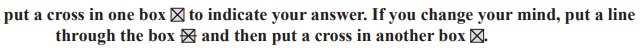
\includegraphics[width=15cm]{Year_6_Mixed_Tests/Xx.png}
\end{center}

\begin{enumerate}

\item \quad  Use the figure below to answer the questions that follow: 

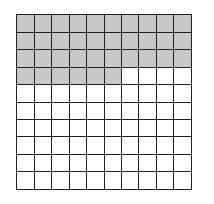
\includegraphics[width=5cm]{Year_6_Mixed_Tests/Homework_Tasks/Shaded_grid_1.png}

(a) What fraction is shaded? Hint - numerator = shaded squares, denominator = all the squares (both shaded and unshaded). \\

(b) What percentage is shaded? Hint - convert the shaded fraction to percentage by multiplying by 100.\\

(c) What fraction is NOT shaded? Hint - numerator =  unshaded squares, denominator = the number of all the squares (both shaded and unshaded).\\

(d) What percentage is NOT shaded? Hint - convert the unshaded fraction to percentage by multiplying by 100. \\

\item \quad \( \framebox(50,15){} + 5,769 = 9,431 \)

\item \quad \( 87,837 = 82,546 + \framebox(50,15){} \)

\item \quad \( 4,586 + 469 = 569 + \framebox(50,15){} \)

\item \quad \( \framebox(50,15){} \div 45 = 53  \)

\item \quad \( 4^{3} - 3^{3} + 1^{3}  \) = \framebox(50,15){}

\item \quad Sort the given numbers into the Venn diagram below. Numbers that fit in both circles are to be put at the point of intersection (the central oval). Numbers that do not belong to any circle should be put in the sample space (between the rectangle and the circles).\hspace{1cm} \( { 1, 2, 3, 4, 8, 9, 27, 64 } \)
\begin{center}
\includegraphics[width=8.5cm]{Year_6_Mixed_Tests/Homework_Tasks/Venn_sq_cb.png}
\end{center}

%\begin{figure}
 %   \centering
  %  \includegraphics[width=0.5\linewidth]{Venn_sq_cb.png}
    %\caption{Enter Caption}
    %\label{fig:enter-label}
%\end{figure}

\end{enumerate}




%\begin{table}
 %   \centering
  %  \begin{tabular}{cccccc}
   %      & 6 & 6 &  &  & \\
    %     &  &  & 9 &  & \\
     %    &  &  &  & 9 & \\
      %   &  &  &  &  & 7 \\
       %  &  &  &  &  & 4 \\
        % &  &  &  &  & 3 \\
    %\end{tabular}
    %\caption{Caption}
    %\label{tab:my_label}
%\end{table}

\end{document}